\documentclass[twocolumn]{article}

\title{Math Cheat Sheet}
\author{Łukasz Komar}
\date{2013-2014}

\usepackage[utf8]{inputenc}
\usepackage{natbib}
\usepackage{amsmath}
\usepackage{graphicx}
\usepackage{multicol}
\usepackage{geometry}
\usepackage{tikz}
\usepackage{hyperref}
\usepackage{lastpage}
\usepackage{fancyhdr}

\usetikzlibrary{calc,matrix}

\geometry{
 a4paper,
 total={210mm,297mm},
 left=5mm,
 right=5mm,
 top=5mm,
 bottom=12mm,
 bindingoffset=0mm
}

\pagestyle{fancy}
\lfoot{\footnotesize{\href{http://github.com/lukaszkomar/math-cheat-sheet}{Łukasz Komar's Math Cheat Sheet}}}
\cfoot{\footnotesize{\href{http://github.com/lukaszkomar/math-cheat-sheet/releases/tag/v1.0.0}{v1.0.0}}}
\rfoot{\footnotesize{\thepage/\pageref{LastPage}}}

\everymath={\displaystyle}
\renewcommand\arraystretch{2}

\begin{document}
\subsection*{\centering{Factoring Formulas}}
\begin{center}
\begin{array}{rcl}
  \mathbf{a^2-b^2}&=&(a-b)(a+b)\\
  
  \mathbf{(a+b)^2}&=&a^2+2ab+b^2\\
  \mathbf{(a-b)^2}&=&a^2-2ab+b^2\\
  
  \mathbf{a^3-b^3}&=&(a-b)(a^2+ab+b^2)\\
  \mathbf{a^3+b^3}&=&(a+b)(a^2-ab+b^2)\\  
  
  \mathbf{(a+b)^3}&=&a^3+3a^2b+3ab^2+b^3\\
  \mathbf{(a-b)^3}&=&a^3-3a^2b+3ab^2-b^3\\
\end{array}
\end{center}
\subsection*{\centering{Radicals}}
\begin{center}
\begin{array}{lclclcl}  
  \sqrt[n]{a}           &=& a^{\frac{1}{n}}                 &\qquad& \sqrt[n]{a^m}         &=& a^{\frac{m}{n}} \\
  \sqrt[n]{\frac{a}{b}} &=& \frac{\sqrt[n]{a}}{\sqrt[n]{b}} &\qquad& \sqrt[n]{a\cdot b}    &=& \sqrt[n]{a}\cdot\sqrt[n]{b} \\
  \sqrt[n]{a^n}         &=& |a|                             &\qquad& \sqrt[m]{\sqrt[n]{a}} &=& \sqrt[m \cdot n]{a}\\  
\end{array}
\end{center}
\subsection*{\centering{Exponents}}
\begin{center}
\begin{array}{lclclcl}  
  a^n\cdot a^m &=& a^{n+m}       &\qquad& \frac{a^n}{a^m}               &=& a^{n-m}\\
  (a\cdot b)^n &=& a^n \cdot b^n &\qquad& \left(\frac{a}{b}\right)^n    &=& \frac{a^n}{b^n}\\
  (a^n)^m      &=& a^{n \cdot m} &\qquad& \left(\frac{a}{b}\right)^{-n} &=& \left(\frac{b}{a}\right)^{n}\\
\end{array}
\end{center}
\subsection*{\centering{Quadratic Formula}}
$$\mathbf{a}x^2+\mathbf{b}x+\mathbf{c} \qquad\textrm{for}\quad a\neq0$$
$$\Delta = b^2-4ac$$
$$x_{1,2}=\frac{-b\pm\sqrt{\Delta}}{2a}$$
$$p=\frac{-b}{2a} \quad , \quad  q=\frac{-\Delta}{4a}$$
$$a(x-p)^2+q \qquad\qquad \textrm{(vertex form)}$$
$$a(x-x_1)(x-x_2) \qquad \textrm{(factored form)}$$
\subsection*{\centering{Logarithms}}
$$a^c=x \Leftrightarrow \log_ax=c \qquad \textrf{for} \qquad a\in\mathbb{R}^{+}_{\setminus\{0\}},  x\in\mathbb{R}^+$$

\begin{center}
\begin{array}{lllll}
  \log_aa               &= 1       &\qquad& \log_a1 &= 0 \\  
  \ln x                 &= \log_ex &\qquad& \log x  &= \log_{10}x \\
  \log_ab \cdot \log_bc &= \log_ac &\qquad& \log_ab &= \frac{1}{\log_ba} \\  
\end{array}
\end{center}

$$\log_a(x\cdot y) &= \log_ax + \log_ay $$
$$\log_a\left(\frac{x}{y}\right) &= \log_ax - \log_ay $$

\subsection*{\centering{Binomial Coefficient}}
$$\binom{n}{k} = \frac{n!}{k!(n-k)!}$$
\subsection*{\centering{Matrices}}
$$
A_{m\times n} =
\[
 \begin{bmatrix}
  a_{1,1} & a_{1,2} & \cdots & a_{1,n} \\
  a_{2,1} & a_{2,2} & \cdots & a_{2,n} \\
  \vdots  & \vdots  & \ddots & \vdots  \\
  a_{m,1} & a_{m,2} & \cdots & a_{m,n}
 \end{bmatrix}
\]
$$

$$
A_{ij} = (-1)^{i+j} M_{ij} \qquad \text{(Cofactor expansion of element $a_{ij}$)}
$$

\noindent Minor $M_{ij}$ is the determinant of submatrix (of rank $n-1$), cut down from $A$ by removing $i$ row and $j$ column.

$$
A^{-1} = \frac{1}{\det A} \cdot [A_{ij}]^T \qquad \text{where}  \qquad A^{-1} \cdot A = A \cdot A^{-1} =  \mathbf{I}
$$

$$
\det A = \sum_{j=1}^{n} a_{ij}A_{ij} \qquad \text{(Laplace expansion)}
$$

$$
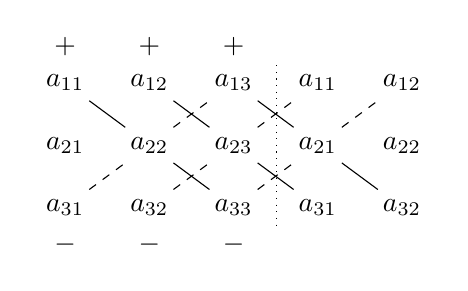
\begin{tikzpicture}
    \matrix [%
      matrix of math nodes,
      column sep=1em,
      row sep=1em
    ] (sarrus) {%
      a_{11} & a_{12} & a_{13} & a_{11} & a_{12} \\
      a_{21} & a_{22} & a_{23} & a_{21} & a_{22} \\
      a_{31} & a_{32} & a_{33} & a_{31} & a_{32} \\
    }; 

    \path ($(sarrus-1-3.north east)+(0.5em,0)$) edge[dotted] ($(sarrus-3-3.south east)+(0.5em,0)$)
          (sarrus-1-1)                          edge         (sarrus-2-2)
          (sarrus-2-2)                          edge         (sarrus-3-3)
          (sarrus-1-2)                          edge         (sarrus-2-3)
          (sarrus-2-3)                          edge         (sarrus-3-4)
          (sarrus-1-3)                          edge         (sarrus-2-4)
          (sarrus-2-4)                          edge         (sarrus-3-5)
          (sarrus-3-1)                          edge[dashed] (sarrus-2-2)
          (sarrus-2-2)                          edge[dashed] (sarrus-1-3)
          (sarrus-3-2)                          edge[dashed] (sarrus-2-3)
          (sarrus-2-3)                          edge[dashed] (sarrus-1-4)
          (sarrus-3-3)                          edge[dashed] (sarrus-2-4)
          (sarrus-2-4)                          edge[dashed] (sarrus-1-5);

    \foreach \c in {1,2,3} {\node[anchor=south] at (sarrus-1-\c.north) {$+$};};
    \foreach \c in {1,2,3} {\node[anchor=north] at (sarrus-3-\c.south) {$-$};};
\end{tikzpicture}
$$

$$\det A = \det A^T$$
$$\det(A \cdot B)=\det A \cdot \det B$$
$$\det (A^{-1})=(\det A)^{-1}$$
$$\det(k \cdot A)=k^n \cdot \det A \qquad k\in\mathbb{R}, n \text{ order of } A$$
\subsection*{\centering{Limits}}
\begin{center}
\begin{array}{lclclcl}
  \lim_{n\to\infty} \frac{1}{n}  &=& 0      &\qquad& \lim_{n\to\infty} \frac{1}{\sqrt{n}}           &=& 0\\
  \lim_{n\to\infty} 2^n          &=& \infty &\qquad& \lim_{n\to\infty} \left(\frac{1}{2}\right)^n   &=& 0 \\  
  \lim_{n\to\infty} n            &=& \infty &\qquad& \lim_{n\to\infty} \left(1+\frac{1}{n}\right)^n &=& e\\    
  \lim_{n\to\infty} \sqrt[n]{a}  &=& 1      &\qquad& \lim_{n\to\infty} \frac{n}{0}                  &=& \infty\\  
  \\
  \lim_{x\to0} \frac{\sin x}{x}  &=& 1      &\qquad& \lim_{x\to0} \left(1+\frac{1}{x}\right)^x      &=& 1 \\    
\end{array}
\end{center}

\subsubsection*{\centering{Indeterminate forms}}
$$
\frac{0}{0}, 
\quad \frac{\infty}{\infty}, 
\quad \infty-\infty, 
\quad 0\cdot\infty, 
\quad \infty^0, 
\quad 1^\infty, 
\quad 0^0
$$
\subsection*{\centering{Derivatives}}
\begin{center}
\begin{array}{lll}
 y=f\Big(g(x)\Big)   &\qquad& y' = f'(g) \cdot g'\\
 y=f(x) \cdot g(x)   &\qquad& y' = f' \cdot g + f \cdot g'\\  
 y=\frac{f(x)}{g(x)} &\qquad& y' = \frac{f' \cdot g - f \cdot g'}{g^2}\\  
\end{array}
\end{center}


\begin{center}
\begin{array}{lllll}
 y=x^n         & y' = n \cdot x^{n-1}         & \qquad\quad & y=ax     & y' = a\\
 y=a^x         & y'=a^x \cdot \ln a           & \qquad\quad & y=e^x    & y'=e^x  \\
 y=\log_{a}{x} & y' = \frac{1}{x \cdot \ln a} & \qquad\quad & y=\ln x  & y'=\frac{1}{x}\\
 y=\sin x      & y'=\cos x                    & \qquad\quad & y=\cos x & y'=-\sin x \\
\end{array}
\end{center}
\end{document}